\section*{Цель}

Исследовать внутреннюю организацию динамического ряда кардиоинтервалов на основе метода корреляционной ритмографии
и автокорреляционного анализа.

\section*{Порядок выполнения}

\begin{enumerate}
    \item По заданному массиву кардиоинтервалов построить график автокоррелограммы.
    \item Рассчитать значение коэффициента корреляции после первого сдвига $СС1$ и число сдвигов до первого нулевого значения коэффициента корреляции $СС0$.
    \item По заданному массиву кардиоинтервалов построить корреляционную ритмограмму.
    \item Проанализировать полученные графики.
\end{enumerate}

\section*{Исходные данные}

В работе используется набор данных из первой лабораторной работы.

\newpage

\section*{Автокорреляционный анализ}

В первую очередь в настоящей лабораторной работе необходимо провести автокорелляционный анализ.
Автокорелляционная функция вычисляется по следующей функции.

\begin{figure}[h!]
    \centering
    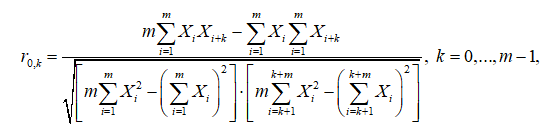
\includegraphics[width=0.8\textwidth]{\jobname/docs/img/autocorellation_func.png}
\end{figure}

На основании найденной автокорелляционной функции также были рассчитаны значения коэффициента корреляции после
первого сдвига $CC1$ и число сдвигов до первого нулевого значения коэффициента корреляции $CC0$.

\begin{align*}
    CC1 & = r_{0,1} = 0.741
\end{align*}

\begin{align*}
    CC0 & = k \frac{\Delta t}{100} = 0.75
\end{align*}

График полученной автокорелляционной функции представлен ниже.

\begin{figure}[h!]
    \centering
    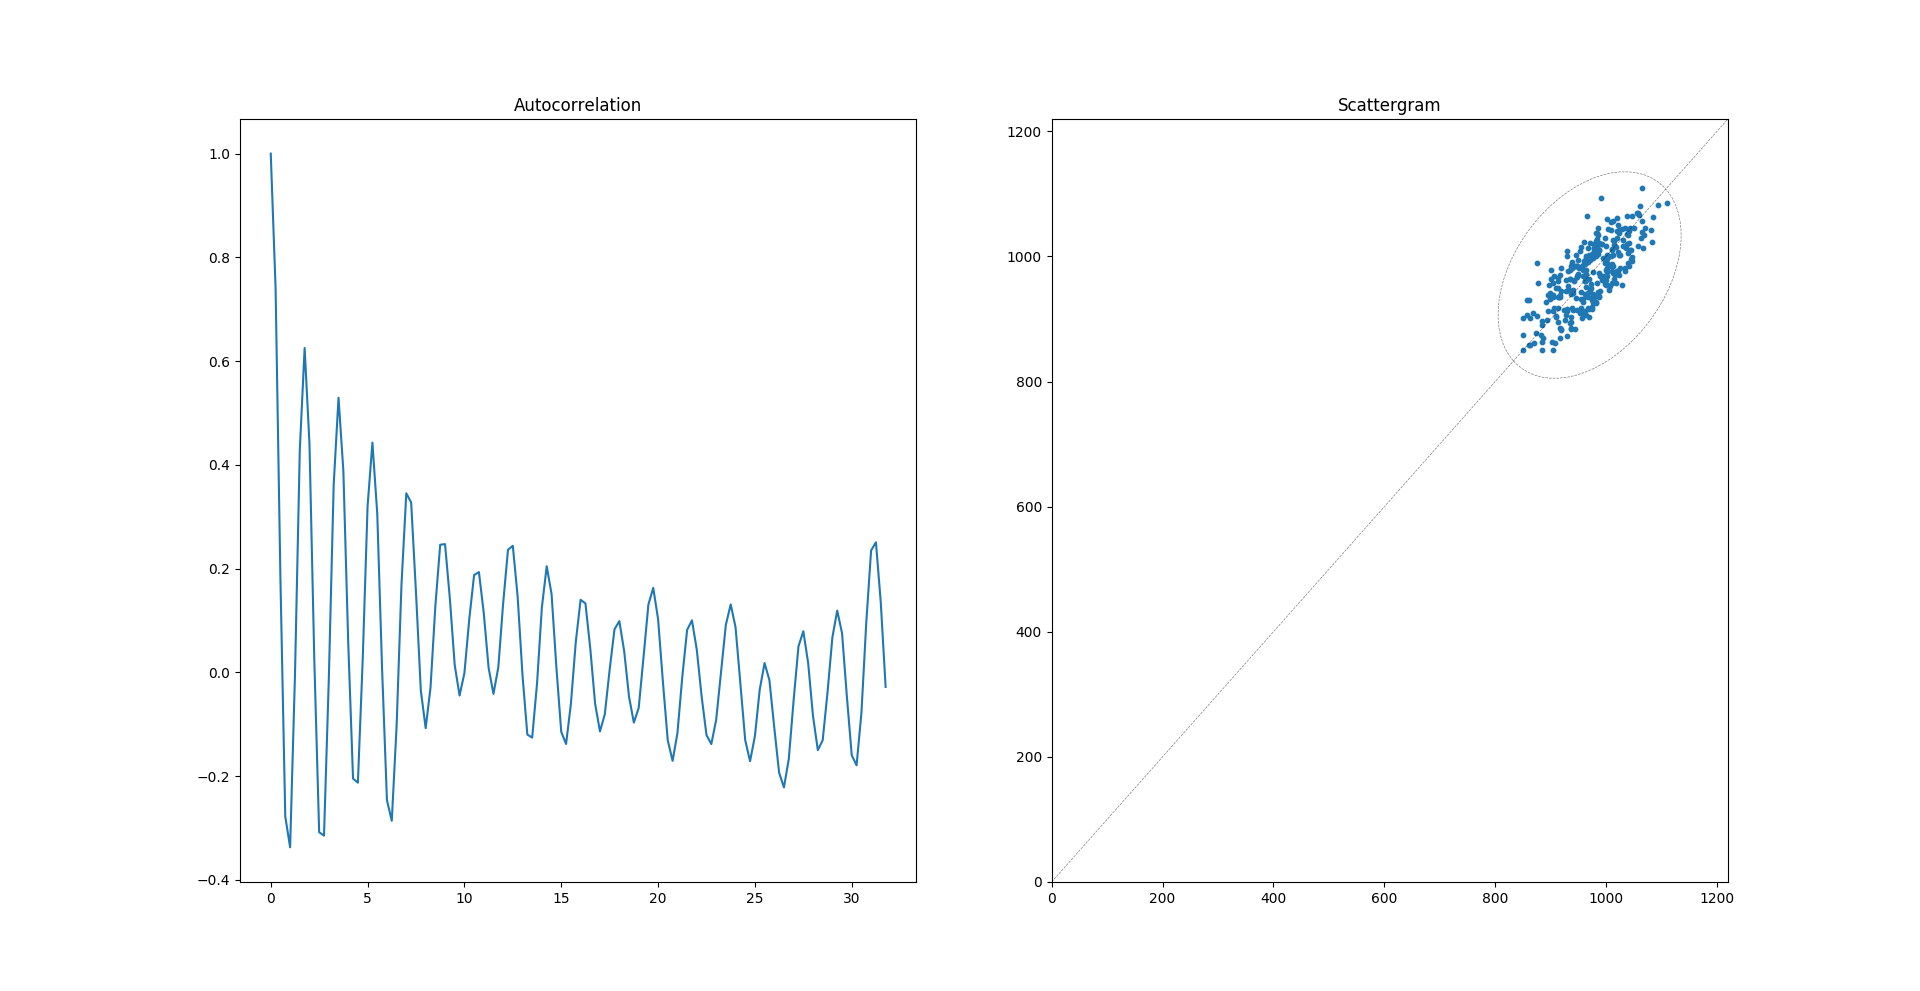
\includegraphics[width=0.8\textwidth]{\jobname/docs/img/graphs.png}
\end{figure}

\section*{Корреляционная ритмография – скаттерография}

Кроме графика автокорелляционной функции выше представлена, т.н. скаттерограмма, отображающая зависимость
последовательных пар кардиоинтервалов.

\clearpage

\section*{Выводы}

В ходе выполнения лабораторной работы был исследован набор входных данных с использованием двух подходов:
автокорреляционный анализа и скаттерографии.

В рамках автокорелляционного анализа была исследована автокорелляционная функция, найдены значения
$CC0$ и $CC1$ равные соответственно 0.75 и 0.741, а также был построен график автокорелляционной функции.

В рамках скаттерографии (корреляционной ритмографии) была построена скаттерограмма.

Полученный график скаттерограммы представляет собой нормальную форму, которая выглядит, как эллипс, вытянутый вдоль
биссектрисы.
Полученное расположение эллипса означает, что к дыхательной прибавлена некоторая величина недыхательной аритмии.
Помимо прочего, учитывая значение числа сдвигов до первого нулевого значения коэффициента корреляции, можно выдвинуть
предположение, что в исследуемой выборке доминируют быстроволновые компоненты.

\clearpage

\section*{Листинги}

\subsection*{Листинг основного скрипта}
\lstinputlisting[language=Python,texcl=true]{\jobname/lab2.py}

\subsection*{Листинг утилитного скрипта}
\lstinputlisting[language=Python,texcl=true]{common/common.py}
